%\title{LaTeX Portrait Poster Template}
%%%%%%%%%%%%%%%%%%%%%%%%%%%%%%%%%%%%%%%%%
% a0poster Portrait Poster
% LaTeX Template
% Version 1.0 (22/06/13)
%
% The a0poster class was created by:
% Gerlinde Kettl and Matthias Weiser (tex@kettl.de)
% 
% This template has been downloaded from:
% http://www.LaTeXTemplates.com
%
% License:
% CC BY-NC-SA 3.0 (http://creativecommons.org/licenses/by-nc-sa/3.0/)
%
%%%%%%%%%%%%%%%%%%%%%%%%%%%%%%%%%%%%%%%%%

%----------------------------------------------------------------------------------------
%	PACKAGES AND OTHER DOCUMENT CONFIGURATIONS
%----------------------------------------------------------------------------------------

\documentclass[a0,portrait,11pt]{a0poster}
\usepackage[utf8]{vietnam}
\usepackage{multicol} % This is so we can have multiple columns of text side-by-side
\columnsep=40pt % This is the amount of white space between the columns in the poster
%\columnseprule=3pt % This is the thickness of the black line between the columns in the poster

\usepackage[svgnames]{xcolor} % Specify colors by their 'svgnames', for a full list of all colors available see here: http://www.latextemplates.com/svgnames-colors

\usepackage{times} % Use the times font
%\usepackage{palatino} % Uncomment to use the Palatino font
\usepackage{longtable}
\usepackage{graphicx} % Required for including images
\graphicspath{{figures/}} % Location of the graphics files
\usepackage{booktabs} % Top and bottom rules for table
\usepackage[font=small,labelfont=bf]{caption} % Required for specifying captions to tables and figures
\usepackage{amsfonts, amsmath, amsthm, amssymb} % For math fonts, symbols and environments
\usepackage{wrapfig} % Allows wrapping text around tables and figures
\usepackage{framed}
\usepackage{xcolor}
\usepackage[framemethod=tikz]{mdframed}
\usepackage{lipsum}
\usepackage{amsmath}
\usepackage{amssymb}
\usepackage[linesnumbered,ruled]{algorithm2e}
\newenvironment{cframed}[1][blue]
  {\def\FrameCommand{\fboxsep=\FrameSep\fcolorbox{#1}{white}}%
    \MakeFramed {\advance\hsize-\width \FrameRestore}}
  {\endMakeFramed}
\definecolor{mycolor}{rgb}{0.122, 0.435, 0.698}
\newmdenv[innerlinewidth=0.5pt, roundcorner=10pt,linecolor=mycolor,innerleftmargin=15pt,
innerrightmargin=15pt,innertopmargin=6pt,innerbottommargin=30pt]{mybox}

\begin{document}
%----------------------------------------------------------------------------------------
%	POSTER HEADER 
%----------------------------------------------------------------------------------------

% The header is divided into two boxes:
% The first is 75% wide and houses the title, subtitle, names, university/organization and contact information
% The second is 25% wide and houses a logo for your university/organization or a photo of you
% The widths of these boxes can be easily edited to accommodate your content as you see fit
\begin{minipage}[b]{0.15\linewidth}

\includegraphics[width=7cm]{hust.jpg}
\end{minipage}
\begin{minipage}[c]{0.73\linewidth}
\begin{center}
\VeryHuge \color{NavyBlue} \textbf{Hệ gợi ý phim} \color{Black}\\ % Title
\Huge\textit{Cài đặt thử nghiệm các thuật toán }\\[2.0cm] % Subtitle
\huge \textbf{Đặng Quang Trung, Trần Bá Thiết}\\[0.5cm] % Author(s)
\huge Đại Học Bách Khoa Hà Nội, Viện công nghệ thông tin và truyền thông, Việt Nam\\[0.4cm] % University/organization
\Large Liên hệ: \texttt{20134145@student.hust.edu.vn}\\
\end{center}
\end{minipage}
%
\begin{minipage}[b]{0.15\linewidth}

\includegraphics[width=7cm]{soict.png}
\end{minipage}

\vspace{2cm} % A bit of extra whitespace between the header and poster content

%----------------------------------------------------------------------------------------

\begin{multicols}{2} % This is how many columns your poster will be broken into, a portrait poster is generally split into 2 columns

%----------------------------------------------------------------------------------------
%	ABSTRACT
%----------------------------------------------------------------------------------------
%
%\color{Navy} % Navy color for the abstract
%
%\begin{abstract}
%The electrical energy from renewables in Algeria contributed about 3.4\% (280 MW) in 2008 of a total power of 8.1 GWe and will reach 5\% by the year 2017 according to the Algerian Electricity and Gas Regulation Commission (CREG). The country’s target is reaching 40\% by 2030. The geothermal resources in Algeria are of low-enthalpy type. Most of these geothermal resources are located in the north of the country and generate a heat discharge of 240 MWt.
%\end{abstract}
%----------------------------------------------------------------------------------------
%	INTRODUCTION
%----------------------------------------------------------------------------------------

\color{Black} % SaddleBrown color for the introduction
\begin{mybox}
\section*{Giới thiệu}
Hằng ngày chúng ta có các ý kiến về những thứ chúng ta thích hoặc không
thích và thậm chí là không quan tâm đến nó. Ví dụ như bạn xem một chương
trình truyền hình trên TV, bạn cảm thấy chương trình rất hay và hài hước
hoặc thấy nó nhàm chán hay bạn không tìm thấy chương trình đó ở tất cả
mọi kênh. Hoặc chương trình đó diễn ra mà chúng ta không để ý. \\ \\
Sở thích của mỗi người là khác nhau, nhưng chúng ta tạo ra các dạng
mẫu người dùng. Mọi người có xu hướng thích những thứ tương tự như những
thứ mà họ thích. \\ \\
Vì thế chúng ta cần có các chiến lược để gợi ý sản phẩm cho người dùng. Ở trình 
hai phương pháp:
\begin{itemize}
\item[•] Collaborative Filtering
\item[•] Latent Factor Model
\end{itemize}
\end{mybox}
\begin{mybox}
\section*{Collaborative Filtering}
\subsubsection*{Ý tưởng basic:}
\begin{minipage}[c]{0.45\linewidth}
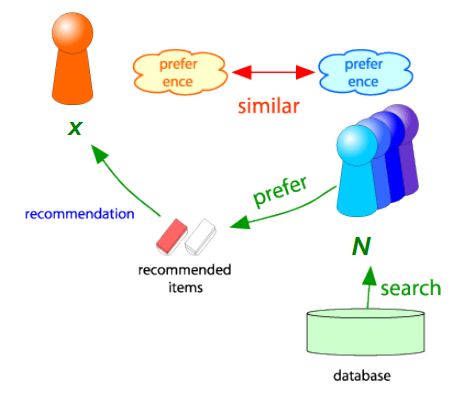
\includegraphics[width=0.8\linewidth]{CF.png}
\end{minipage}
\begin{minipage}[b]{0.45\linewidth}
\begin{itemize}
\item[•] quan sát một người dùng x.
\item[•] Tìm tập N các người dùng khác cũng rating giống như các ratings của
người dùng x.
\item[•] Ước lượng các ratings của người dùng x dựa trên các ratings của những
người trong tập N.
\end{itemize}
\end{minipage}
\subsubsection*{Tìm tập người tương đồng:}
\begin{itemize}
\item[•] Độ đo tương đồng Cosine
\begin{itemize}
\item[-] $sim(x,y) = \cos(\vec{r}_x , \vec{r}_y) = \frac{\vec{r}_x.\vec{r}_y}{\parallel \vec{r}_x \parallel . \parallel \vec{r}_y \parallel}$
\item[-] Vấn đề: khắc phục được nhược điểm của jaccard nhưng lại bỏ qua các ratings không tốt(người dùng đánh giá thấp bộ phim đó)
\end{itemize}
\item[•] Sử dụng hệ số tương phản cá nhân
\begin{itemize}
\item[-] $S_{xy}$ là tập các bộ phim được rating bởi x và y.
\small{
\item[-] $sim(x,,y) = \sum s\in S\downarrow xy \uparrow (r\downarrow xs - r\downarrow x)r\downarrow ys - r\downarrow y)/\sqrt{\sum s\in S\downarrow xy \uparrow (r\downarrow xs - r\downarrow x)\uparrow 2}$
}
\end{itemize}
\end{itemize}
\subsection*{Dự đoán rating người dùng:}
\begin{center}
\Large{
$\hat{r_{xi}} = b_{xi} + \frac{\sum_{j\in N(i;x)}s_{ị}.(r_{xj} - b_{xj})}{\sum_{j\in N(i;x)}s_{ị} }$
}
\end{center}
Với $b_{xi} = \mu + b_x + b_i$ là độ lệch cơ sở của người dùng x khi đánh giá bộ phim i. Trong đó:
\begin{itemize}
\item[-] $\mu$ là rating trung bình của tất cả người dùng.
\item[-] $b_x$ là độ lệch của người dùng x.
\begin{itemize}
\item[] $b_x = avg(x) - \mu $.
\end{itemize}
\item[-] $b_i$ là độ lệch của bộ phim i.
\begin{itemize}
\item[] $b_i = avg(i) - \mu $.
\end{itemize}
\end{itemize}
\end{mybox}
\begin{mybox}
\section*{Latent Factor Models}
\subsection*{Ý tưởng:}
Trong thức tế mỗi người dùng sẽ có những sở thích riêng của mình ví dụ như có người thích phim tình cảm, lãng mạn có người thích phim hành động, khoa học viễn tưởng, \ldots . Những sở thích đó được coi là một nhân tố ẩn của mỗi người dùng. \\ \\
\begin{minipage}[c]{0.45\linewidth}
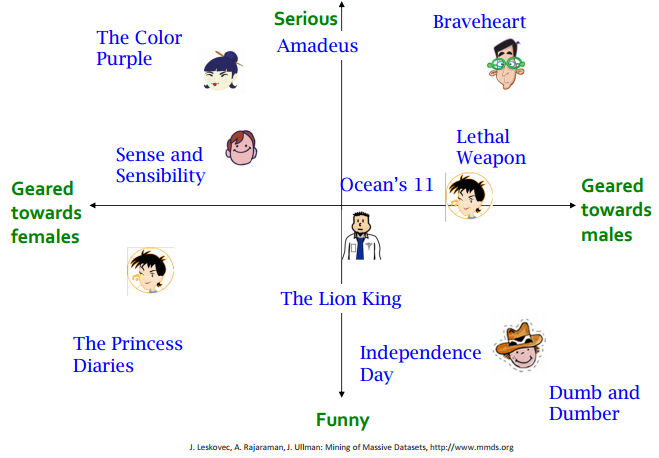
\includegraphics[width=0.8\linewidth]{LF.png}
\end{minipage}
\begin{minipage}[c]{0.45\linewidth}
\begin{itemize}
\item[•] Các ratings chịu ảnh hưởng sâu sắc bởi một bộ các nhân tố(factor) rất cụ thể cho miền.
\item[•] Một số các factors là rất khó quan sát được và khó ước lượng sự tác động của chúng đối với ratings của người dùng.
\item[•] Mục tiêu là suy luận những nhân tố tiềm ẩn từ dữ liệu đánh giá bằng cách sử dụng các kỹ thuật toán học.
\end{itemize}
\end{minipage}
\subsubsection*{SVD:}
\begin{minipage}[c]{0.5\linewidth}
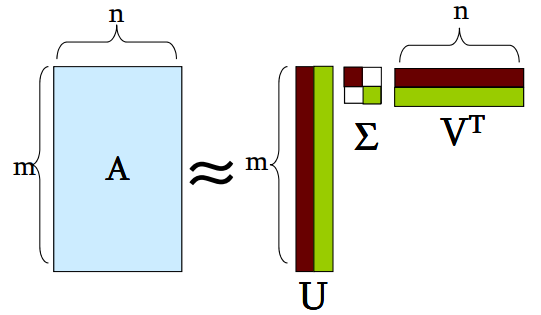
\includegraphics[width=18cm]{svd.png}
\captionof{figure}{\color{Green}Hình ảnh minh họa svd}
\end{minipage}
\begin{minipage}[c]{0.4\linewidth}
Trong đó:
\begin{itemize}
\item[-] U là ma trận vói các cột là các vector trái.
\item[-] S là ma trận cùng kích thước như A giá trị đợn là đường chéo.
\item[-] $V^T$ có các hàng là cá vector đơn phải 
\end{itemize}
\end{minipage}
\subsection*{Dự đoán rating người dùng:}
\begin{minipage}[c]{0.6\linewidth}
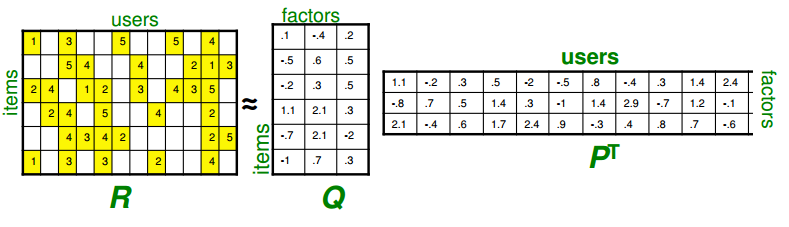
\includegraphics[width=20cm]{svd1.png}
\captionof{figure}{\color{Green}Ma trận sau khi giảm chiều sử dụng svd}
\end{minipage}
\begin{minipage}[c]{0.4\linewidth}
Trong đó:
\begin{itemize}
\item[•] A = R là ma trận người dùng ban đầu.
\item[•] Q là ma trận nhân tố của phim.
\item[•] $P^T$ là ma trận nhân tố của người dùng.
\begin{itemize}
\item[] $P^T = \sum V^T$
\end{itemize}
\end{itemize}
\end{minipage}
Để dự đoán rating của người dùng x cho một bộ phim ra chỉ cần tính:
\begin{center}
\begin{center}
$r_{xi} = \underbrace{\mu}_{overall mean rating} + \underbrace{b_{x}}_{bias for user x} + \underbrace{b_{i}}_{bias for moive i} + q_{x}.p_i$
\end{center}
\end{center}
Trong đó:
\begin{itemize}
\item[-] $q_i$ là hàng i của ma trận Q.
\item[-] $p_x$ là cột x của ma trận P.
\item[-] f là số factors(hay độ dài vector của hàng i và cột x).
\end{itemize}
\subsection*{Vấn đề tối thiểu hóa lỗi và overfitting:}
%Như đã biết SVD đã tối thiếu hóa lỗi trên toàn ma trận để ít mất mát thông tin nhất.Chúng ta có thể xây dựng lại hàm lỗi:
\begin{minipage}[c]{0.6\linewidth}
\begin{flushleft}
\begin{displaymath}
\displaystyle \min_{Q,P} \sum_{(x,i)\in R}(r_{xi} - (\mu + b_x + b_i + q_i.p_x))^2
\end{displaymath}
\end{flushleft}
\begin{center}
\begin{displaymath}
\displaystyle
+ (\lambda_1\sum_{i}\Vert q_i \Vert^{2} + \lambda_2\sum_x\Vert p_x \Vert^2 + \lambda_3\sum_x\Vert b_x \Vert^2 + \lambda_4\sum_i\Vert b_i \Vert^2)
\end{displaymath}
\end{center}
\end{minipage}
\begin{minipage}[c]{0.4\linewidth}
Trong đó:
\begin{itemize}
\item[-] $\lambda_1,\lambda_2,\lambda_3,\lambda_4$ là các hệ số phạt.
\begin{itemize}
\item[+] Để đơn giản ở đây tất cả dùng chung $\lambda$
\end{itemize}
\item[-] $b_i,b_x$ là độ lệch của moive và người dùng.
\item[-] $\mu$ là raitng trung bình của ma trận người dùng.
\item[-] $q_i,p_x$ là các vector hàng và cột của ma trận Q,P.
\end{itemize}
\end{minipage}
\end{mybox}
%----------------------------------------------------------------------------------------
%	REFERENCES
%----------------------------------------------------------------------------------------

\nocite{*} % Print all references regardless of whether they were cited in the poster or not
\bibliographystyle{plain} % Plain referencing style
\bibliography{sample} % Use the example bibliography file sample.bib

%----------------------------------------------------------------------------------------
\end{multicols}
\begin{mybox}
\section*{Kết quả thực nghiệm}
\begin{multicols}{3}
\subsection*{Collaborative:}
\begin{center}
\begin{tabular}{|c|c|c|}
\hline
Bộ dư liệu & k(hàng xóm) & RMSE \\ 
\hline
ml-100k & 3 &  0.9928 \\
ml-100k & 10 &  0.9236\\
ml-100k & 15 &  0.921\\
ml-100k & 5 & 0.9537 \\
ml-1m & 5 & 0.8835 \\
\hline
\end{tabular}
\end{center}
\subsection*{Latent factor model:}
\begin{center}
\begin{tabular}{|l|l|l|l|}
\hline
Bộ dữ liệu & k(factor) & n\_eopchs & RMSE \\
\hline
ml-100k & 40 & 100 & 0.9161 \\
ml-1m & 40 & 45 & 0.8626 \\
\hline
\end{tabular}
\end{center}
\begin{minipage}[c]{0.5\linewidth}
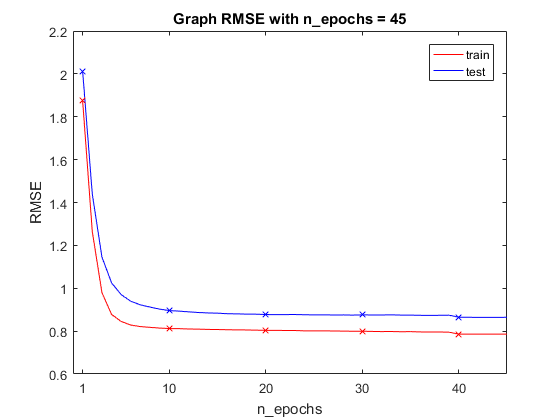
\includegraphics[width=1.0\linewidth]{RMSE!.png}
\captionof{figure}{\color{Green}Hình ảnh RMSE với tập dữ liệu ml-100k}
\end{minipage}
\begin{minipage}[c]{0.5\linewidth}
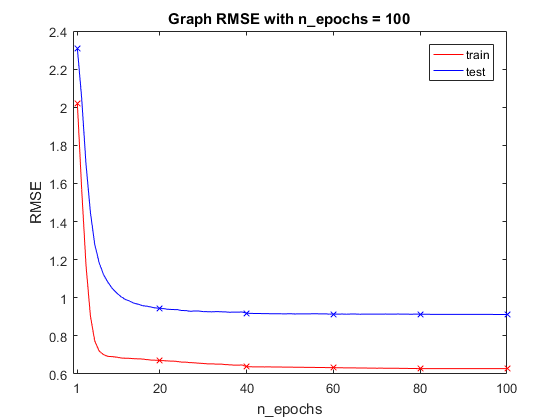
\includegraphics[width=1.0\linewidth]{RMSE.png}
\captionof{figure}{\color{Green}Hình ảnh RMSE với tập dữ liệu ml-1m}
\end{minipage}
\begin{minipage}[c]{0.5\linewidth}
\end{minipage}
\subsection*{Kết luận:}
\begin{itemize}
\item[•] Cả hai phương pháp dễ tiếp cận và cài đặt trong thực tiễn.
\item[•] Qua thực nghiệm thấy rằng Latent cho kết quả tốt hơn Collaborative Filltering basic
\end{itemize}
\end{multicols}
\end{mybox}
\begin{center}
\begin{minipage}[c]{0.6\linewidth}
\begin{mdframed}[backgroundcolor=gray!20]
\begin{center}
   Nội dung của poster này về hê gợi ý môn học khai phá web, mã học phần IT4868
\end{center}
\end{mdframed}
\end{minipage}
\end{center}
\end{document}